\chapter[Implementación]{Implementación}
\label{cp:implementation}

\parindent0pt

La fase de implementación representa el proceso de traducción del diseño de \gls{software} a código ejecutable, constituyendo el puente entre la teoría y la práctica. En el marco del modelo en V, este proceso es una de las etapas finales de la fase descendente, que a su vez marca el inicio de la fase ascendente, ya que la implementación de cada módulo va acompañada de la ejecución de pruebas unitarias. Este enfoque iterativo de desarrollo y validación temprana busca asegurar que la funcionalidad de cada componente se verifique de forma continua para minimizar la aparición de errores cuando el software se despliegue en un entorno real. El proceso de implementación implica tanto la escritura de código, como también la integración de los distintos módulos del sistema, la documentación del código y la preparación del entorno para el despliegue.

La implementación del software se llevó a cabo siguiendo la planificación elaborada a partir de las historias de usuario junto con el diseño del sistema. Durante la ejecución de esta etapa, se utilizó la herramienta Jira para gestionar las tareas en curso y el progreso del desarrollo. El cronograma original enfrentó desviaciones debido a la superposición de actividades académicas y compromisos imprevistos, pero la flexibilidad en la gestión del proyecto permitió la adaptación, posibilitando el cumplimiento de los objetivos del trabajo. En esta fase de desarrollo, se implementa e integra cada uno de los módulos definidos en el proceso de diseño, asegurando su funcionamiento de forma aislada y en conjunto.

El proceso de desarrollo se estructuró para seguir un flujo de trabajo lógico. En primer lugar, se crearon los \glspl{contratointeligente}, que conforman la capa más interna del prototipo y definen la lógica de las transacciones en la \textit{blockchain}. Posteriormente, se construyó la API, que actúa como intermediario para interactuar con los contratos. Finalmente, se desarrolló la interfaz de usuario, que sirve como la capa de presentación. Este enfoque se adoptó con el objetivo de garantizar que cada componente estuviera operativo y probado antes de proceder a la siguiente capa que interactúa con él. A nivel de dominio, el desarrollo siguió secuencialmente el ciclo de vida del vidrio (productor primario, secundario, consumidor, reciclador) para mantener la coherencia del sistema. En la siguiente sección se detalla el proceso de generación de código llevado a cabo durante la implementación del prototipo (Sección \ref{sec:code-generation}). Seguidamente, se describe el proceso de despliegue del sistema en un entorno de pruebas para ser utilizado en las etapas de validación posteriores (Sección \ref{sec:deployment}). Finalmente, se aborda la estrategia de documentación del software desarrollado (Sección \ref{sec:documentation}).

\section{Generación de código}
\label{sec:code-generation}

La implementación del prototipo se realizó en un entorno de desarrollo local, siguiendo un flujo de trabajo que priorizó la separación por capas para gestionar las dependencias del sistema. Como la lógica de negocio central recae en los \glspl{contratointeligente}, su implementación fue la primera en abordarse. La capa de datos no solo define la lógica de las transacciones en la \textit{blockchain}, sino que también establece el modelo de datos base que utilizan las capas superiores. Una vez que los contratos estuvieron completamente desarrollados y probados en base a las especificaciones de requerimientos y diseño, se procedió a la construcción de la API. Esta capa actúa como un intermediario entre los contratos y el \textit{\gls{frontend}}, siendo responsable de traducir las peticiones de la interfaz de usuario en transacciones y llamadas a los contratos. Finalmente, se construyó la interfaz de usuario, que se conecta a la API para poder presentar la información al usuario y permitir la interacción con el sistema.

Para cada funcionalidad del sistema, es posible identificar un flujo de trabajo común que se repite en cada módulo. En primer lugar, se desarrolla la función correspondiente en los contratos inteligentes, como se puede ver en el Código \ref{listing:solidity-create-batch-code} con la función para crear un lote de botellas de vidrio, que recibe los parámetros necesarios, crea un nuevo lote y lo almacena en la \textit{blockchain}, emitiendo un evento para notificar su creación. A continuación, se escribe un \textit{\gls{endpoint}} en la API que llama a esta función del \gls{contratointeligente}, tal como se puede observar en el Código \ref{listing:api-create-batch-code}, que contiene la implementación del repositorio de este \textit{endpoint}. Finalmente, se implementa la interfaz de usuario que permite a los usuarios finales interactuar con esta funcionalidad a través de un formulario con un botón de envío, como se muestra en el Código \ref{listing:frontend-create-batch-code} con el componente de React que maneja la creación del lote de botellas. Este componente recoge los datos del formulario, llama a un servicio que envía una solicitud a la API y maneja la respuesta para proporcionar mensajes de retroalimentación al usuario. Durante la ejecución de este código, el flujo comienza en el \textit{frontend}, que envía una solicitud a la API cuando el usuario presiona el botón para crear un lote. La API procesa esta solicitud y llama a la función correspondiente en el contrato inteligente, que ejecuta la lógica de negocio y actualiza el estado en la \textit{blockchain}, emitiendo eventos que la API puede escuchar para actualizar la \gls{basededatos} relacional con la información del nuevo lote creado. 

\begin{listing}[!tb]
\caption{Función para la creación de un lote de botellas de vidrio en la blockchain (Solidity)}
\label{listing:solidity-create-batch-code}
\begin{minted}{typescript}
function createBaseBottlesBatch(uint256 quantity, Bottle memory bottleType, address owner, string memory createdAt) external onlyContractOwner {
  BaseBottlesBatch memory newBatch = BaseBottlesBatch({
    id: nextBatchId,
    quantity: quantity,
    bottleType: bottleType,
    owner: owner,
    soldQuantity: 0,
    createdAt: createdAt,
    deletedAt: ""
  });

  baseBottlesBatches[nextBatchId] = newBatch;
  emit BaseBatchCreated(nextBatchId, owner);
  nextBatchId++;
}
\end{minted}
\end{listing}

\begin{listing}[!tb]
\caption{Función del repositorio de la API para la creación de un lote de botellas de vidrio (Node.js)}
\label{listing:api-create-batch-code}
\begin{minted}{typescript}
async function CreateBaseBottlesBatch(
  batch: BaseBottlesBatch,
): IResult<number> {
  const createdAt = new Date().toISOString();
  const result = await this.callContractMethod(
    'createBaseBottlesBatch',
    batch.quantity,
    batch.bottleType,
    batch.owner,
    createdAt,
  );
  if (!result.ok) return result;

  // Get created batch id from events emmited or default to 0.
  const batchId = result.data.find((event) => event.name === 'BaseBatchCreated')?.batchId ?? 0;

  return { ok: true, status: StatusCodes.OK, data: batchId };
}
\end{minted}
\end{listing}

\begin{listing}[!tb]
\caption{Función para la creación de un lote de botellas de vidrio en el frontend (Next.js)}
\label{listing:frontend-create-batch-code}
\begin{minted}{typescript}
function CreateBaseBottlesBatchButton = ({ form }): Props {
  async function handleSubmit() {
    const payload = data;
    const { ok } = await createBatchService(payload);
    if (ok) {
      toast.success('Lote de botellas creado correctamente');
    } else {
      toast.error('Ocurrió un error al crear el lote de botellas');
    }
  };

  async function createBatchService(data: BottleBatch) {
    try {
      const res = await fetch(`/producer/batch`, {
        method: 'POST',
        body: JSON.stringify(data),
      });
      const data = await res.json();
      return { ok: true, data: data.batchId };
    } catch {
      return { ok: false, data: null };
    }
  }

  return (
    <button type="submit" onClick={handleSubmit}>Crear Lote</button>
  );
}
\end{minted}
\end{listing}

El proceso de desarrollo se concibió de manera iterativa, donde la escritura de código se alternó con la creación de pruebas unitarias. Este método permitió verificar el correcto funcionamiento de cada componente de forma individual, asegurando que las funciones y módulos cumplieran con las especificaciones de diseño. Gracias al diseño de sistema realizado previamente, la implementación de cada módulo se llevó a cabo de manera sistemática sin bloqueos, pero esto no implicó que no surgieran desafíos técnicos durante la integración de los componentes. Un ejemplo destacable durante la implementación fue el desafío de adaptar la API a la naturaleza inherente de los \glspl{contratointeligente}, los cuales no retornan datos de forma nativa, sino que emiten eventos notificando cambios en su estado. Esta particularidad técnica de la \textit{blockchain} requirió que la capa de la API fuera adaptada para escuchar estos eventos, capturando información como los identificadores únicos de los lotes de vidrio recién creados para su posterior almacenamiento en la base de datos relacional. Esta solución técnica permitió demostrar la viabilidad de la arquitectura híbrida propuesta, asegurando la sincronización de la información entre la \textit{blockchain} y la base de datos complementaria. 

A nivel de dominio, la implementación de las funcionalidades siguió el ciclo de vida del vidrio para mantener una mayor coherencia. El desarrollo se inició con las funcionalidades del productor primario, continuó con las del productor secundario, luego con las del consumidor y, finalmente, con las del centro de reciclaje, cerrando así el ciclo de \gls{trazabilidad}. Una vez que se completaron las funcionalidades para cada actor, se desarrolló la funcionalidad de seguimiento de extremo a extremo, que permite visualizar el historial completo de un envase desde su producción hasta su revalorización. Este enfoque permitió que el flujo del proceso de trazabilidad se construyera de manera lógica y progresiva. Una vez que todas las funcionalidades del prototipo fueron implementadas a nivel de código, se procedió a realizar el despliegue del prototipo en un entorno de pruebas, como se detalla en la siguiente sección.

\section{Despliegue}
\label{sec:deployment}

Una vez que cada módulo del sistema fue implementado y verificado con pruebas unitarias en un entorno local, se procedió a realizar un despliegue del sistema en un entorno de pruebas de características similares a un entorno productivo real. El objetivo principal de esta acción fue demostrar la operatividad del prototipo y proveer un entorno estable y accesible en línea para utilizar en las etapas de pruebas de sistema y pruebas de aceptación. Para ello, se eligieron plataformas gratuitas que permitieran la exposición pública de los componentes del sistema, lo cual facilitó la validación por parte de terceros y la demostración de la viabilidad del proyecto dentro del alcance de un trabajo académico.

En primer lugar, para la modularización y gestión del despliegue, se configuraron contenedores de Docker\footnote{\url{https://docker.com/}} para cada uno de los componentes del sistema. El uso de esta tecnología permitió empaquetar la aplicación y sus dependencias en unidades portables y autónomas, para poder garantizar la reproducibilidad del trabajo en cualquier entorno y facilitar la futura transición del prototipo a un entorno productivo evitando problemas de compatibilidad debido a diferencias en la configuración del entorno. Por ejemplo, el contenedor de la API incluye el servidor Node.js junto con las dependencias del proyecto y puede construirse y ejecutarse utilizando los comandos listados en el Código \ref{listing:docker-api-commands} utilizando variables de entorno para configurar parámetros como el puerto para el servicio y las credenciales de la base de datos.

\begin{listing}[!htb]
\caption{Comandos para construir y ejecutar el contenedor de la API con Docker}
\label{listing:docker-api-commands}
\begin{minted}{bash}
# Build the Docker image
docker build -t $DOCKER_TAG .

# Run the Docker container
docker run -d -e PORT -e DB_HOST -e DB_PORT -e DB_USER -e DB_PASS \
 -e FIREBASE_CONFIG -e PRIVATE_KEY -e PROVIDER_URL -e BASE_BATCH_CONTRACT_ADDRESS \
 -e PRODUCT_BATCH_CONTRACT_ADDRESS -e RECYCLING_CONTRACT_ADDRESS \
 -p $EXTERNAL_PORT:$PORT --name $DOCKER_TAG $DOCKER_TAG
\end{minted}
\end{listing}


Posteriormente, el despliegue se llevó a cabo de forma diferente para cada tecnología. La API de \textit{\gls{backend}} se desplegó en una plataforma de alojamiento web \footnote{\url{https://cloud.google.com/}}, los \glspl{contratointeligente} se publicaron en una red de pruebas de Ethereum \footnote{\url{https://sepolia-optimism.etherscan.io/}} y la interfaz de usuario se puso a disposición en un servicio de hospedaje web estático \footnote{\url{https://vercel.com/}}. Esta configuración logró que el prototipo fuera accesible en línea y a su vez permitió la ejecución de pruebas de integración y aceptación de usuarios en un entorno que replicaba las condiciones de uso finales. Si bien el prototipo se implementó en un entorno de pruebas, fue diseñado con una arquitectura escalable, con el objetivo de facilitar una transición sin fricciones a un entorno productivo en el futuro.

Finalmente, todos los detalles del proceso de despliegue, incluyendo las instrucciones para la configuración del entorno local y la replicación del despliegue en producción, se documentaron exhaustivamente en cada repositorio del proyecto. Esta documentación asegura que otros desarrolladores o investigadores puedan reproducir el entorno de desarrollo y desplegar el sistema de manera autónoma, contribuyendo a la transparencia y accesibilidad del trabajo realizado. En la siguiente sección se detalla la estrategia de documentación adoptada para el prototipo desarrollado.

\section{Documentación}
\label{sec:documentation}

Como parte integral del proceso de \gls{ingenieriadesoftware}, la documentación busca asegurar la mantenibilidad del código, facilitar la colaboración futura y consolidar el conocimiento técnico del proyecto. En este trabajo, el prototipo se documentó en tres niveles: la documentación del código fuente, la interfaz de la API y la configuración del proyecto.

En el primer nivel, se incluyeron comentarios directamente en el código fuente de cada repositorio, tanto en los contratos inteligentes, como en la API y el \textit{\gls{frontend}}. Esto permite que el código sea autoexplicativo y más fácil de comprender para otros desarrolladores o para futuros trabajos de mantenimiento. 

En el segundo nivel, se utilizó la especificación de OpenAPI \footnote{Estándar OpenAPI: \url{https://swagger.io/specification/}} para describir la interfaz de la API del \textit{\gls{backend}}, detallando todos los \textit{endpoints}, parámetros y formatos de solicitudes y respuestas. A partir de este estándar, se utilizó una librería para generar un sitio web interactivo que presenta esta documentación de manera accesible. Exponer esta documentación facilita que la API sea interoperable y pueda ser consumida por cualquier otra aplicación cliente, por ejemplo, en el caso de que se desarrollen nuevas interfaces de usuario o aplicaciones móviles que se conecten a la misma API. 

En la Figura \ref{fig:openapi-docs} se puede observar una captura de pantalla del sitio web con la documentación del \textit{\gls{endpoint}} de creación de lotes de botellas. Este sitio web fue generado automáticamente a partir de la especificación OpenAPI implementada en el Código \ref{listing:openapi-create-batch-code} y contiene información sobre el \textit{endpoint} como el método HTTP, la \gls{url}, los parámetros esperados, los códigos de respuesta y ejemplos de solicitudes. Esta documentación interactiva sirve como referencia para desarrolladores que deseen integrar o extender la funcionalidad de la API, proporcionando una guía clara y confiable sobre cómo interactuar con el sistema.

\begin{listing}[!htb]
\caption{Descripción del endpoint para crear un lote de botellas mediante el estándar OpenAPI}
\label{listing:openapi-create-batch-code}
\begin{minted}{typescript}
/** 
 * POST /producer/batch
 * @summary Crea un nuevo lote de botellas base
 * @tags 2. Productor Primario - Operaciones para productores de botellas
 * @param {CreateBaseBottlesBatchRequest} request.body.required - Datos del lote
 * @security BearerAuth
 * @return {CreationResponse} 201 - Lote creado exitosamente
 * @return {ErrorResponse400} 400 - Datos de lote inválidos
 * @return {ErrorResponse401} 401 - No autorizado
 * @example request - Ejemplo de lote
 * {
 *   "quantity": 100,
 *   "bottleType": {
 *     "weight": 500,
 *     "color": "Verde",
 *     "thickness": 2,
 *     "shapeType": "Cuello alto",
 *     "originLocation": "Argentina",
 *     "extraInfo": "Vidrio reciclado",
 *     "composition": [{ "name": "Calcín", "amount": 100, "measureUnit": "%" }]
 *   },
 *   "createdAt": "2025-05-22T10:00:00Z"
 * } 
 */
async function CreateBaseBottlesBatch(req: Request, res: Response) { 
  /* Código del router... */ 
}
\end{minted}
\end{listing}

\begin{figure}[!htb]
	\centering
	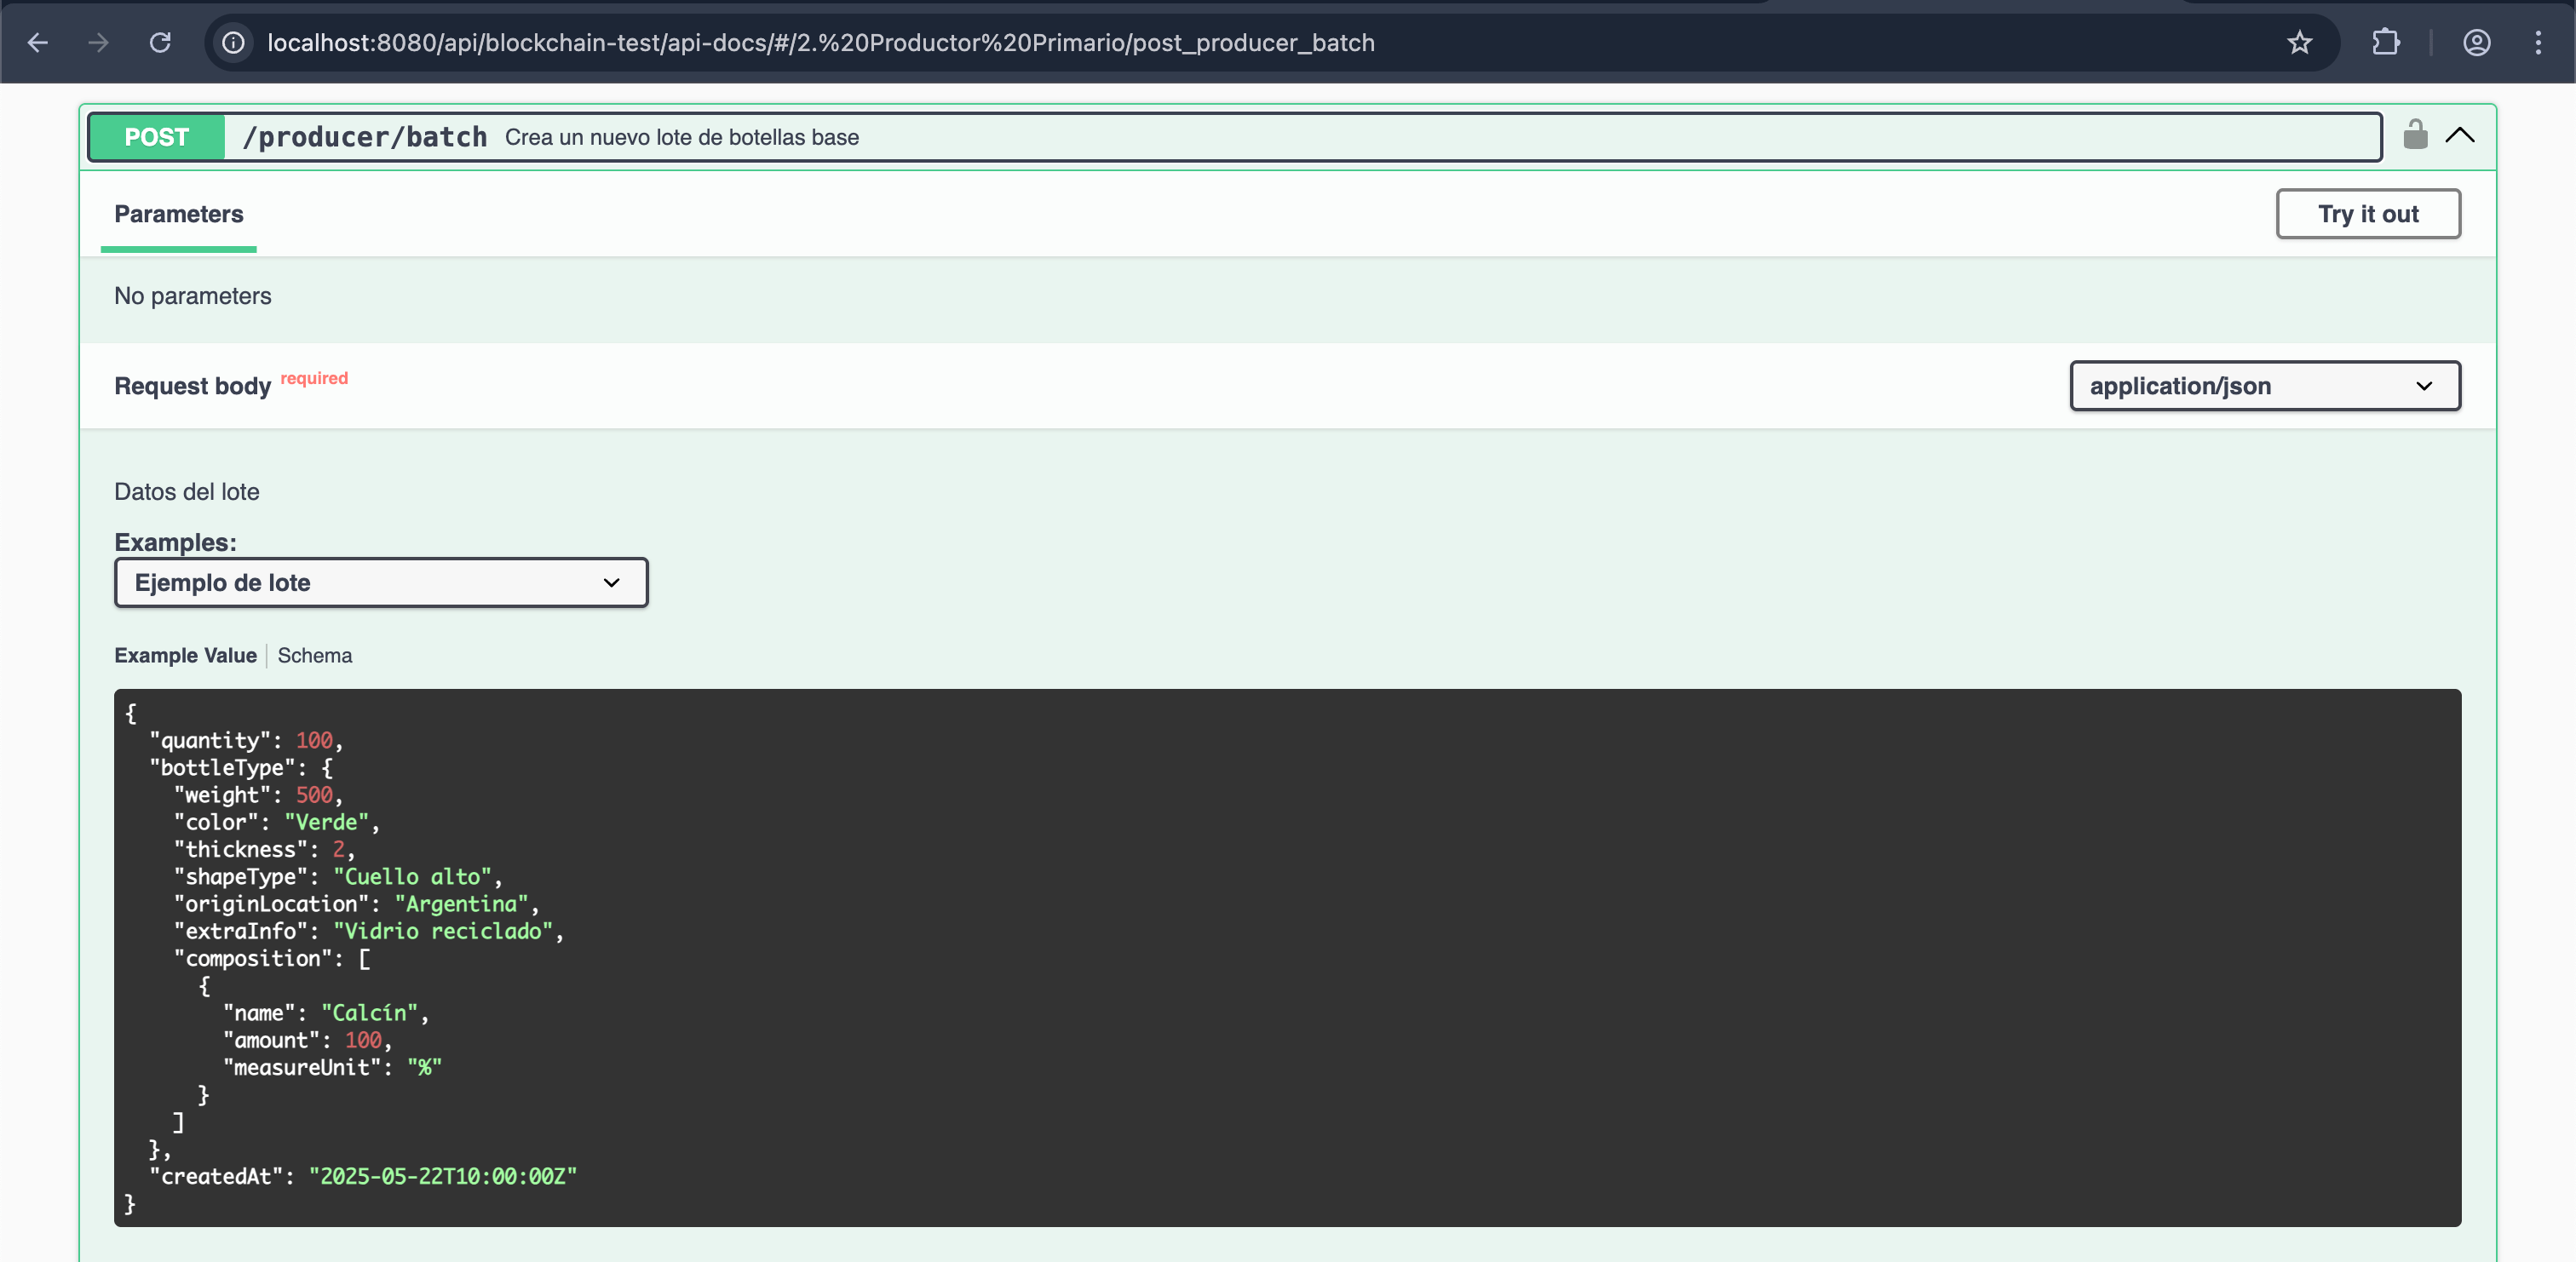
\includegraphics[width=\textwidth]{Figures/openapi-endpoint.png}
	\caption{Documentación interactiva del \textit{\gls{endpoint}} para crear un lote de botellas generada automáticamente a partir de la especificación OpenAPI}
	\label{fig:openapi-docs}
\end{figure}

Finalmente, en el tercer nivel, cada repositorio cuenta con un archivo \textit{README} que actúa como una guía de referencia rápida para la configuración y operación del sistema. Estos archivos detallan los requisitos técnicos, la estructura del proyecto y los comandos para ejecutar pruebas y desplegar el sistema. A su vez, también se incluyó una explicación de la arquitectura de cada repositorio y una serie de enlaces de utilidad que pueden ser de ayuda para los desarrolladores que comiencen a interactuar con el código del proyecto.

Concluido el proceso de implementación y documentación del código, el prototipo del sistema de trazabilidad del vidrio se considera listo para la fase de validación. La construcción de cada componente, desde los contratos inteligentes hasta la interfaz de usuario, ha sido exhaustivamente verificada con pruebas unitarias, sentando las bases para una evaluación más rigurosa. El siguiente capítulo abordará en detalle el proceso de verificación del sistema, detallando la metodología de pruebas unitarias, de integración, de sistema y de aceptación del usuario para asegurar la calidad y el correcto funcionamiento del prototipo en su conjunto.
